\documentclass[12pt,a4paper]{report}

% We don't use it because xelatex support unicode by default
%\usepackage[utf8]{inputenc}  %mettre latin1 à la place de utf8 si vous utilisez latin1
\usepackage{pdfpages}
\usepackage[T1]{fontenc}
\usepackage[utf8]{inputenc}
\usepackage{microtype}
\usepackage{setspace}
\usepackage[sfdefault]{carlito}
\usepackage{listings}
\usepackage{xcolor}

% Define YAML style
\lstdefinelanguage{YAML}{
	keywords={true,false,null,y,n},
	keywordstyle=\color{darkgray}\bfseries,
	sensitive=false,
	comment=[l]{\#},
	morecomment=[s]{/*}{*/},
	commentstyle=\color{purple}\ttfamily,
	stringstyle=\color{red}\ttfamily,
	morestring=[b]',
	morestring=[b]"
}
% Set the global style for listings
\lstset{
	basicstyle=\small\ttfamily,
	numbers=left,
	numberstyle=\tiny,
	numbersep=5pt,
	showstringspaces=false,
	breaklines=true,
	frame=tb,
	backgroundcolor=\color{gray!10},
	breakautoindent=true,
	captionpos=b
}

\renewcommand{\baselinestretch}{0}
\usepackage[french, english]{babel}   %langue française et anglais. Si vous utilisez d'autres langues, ajoutez-les ici. Quand vous avez du texte en anglais, il faut ajouter la commande \selectlanguage{english}. Après, rappelez-vous de revenir au français avec \selectlanguage{french}
\usepackage[maxlevel=3]{csquotes}
\usepackage[backend=biber,style=numeric,isbn=false,sorting=none]{biblatex}
%\usepackage{droit-fr}
\DefineBibliographyStrings{french}{in={dans},inseries={dans}}
\addbibresource{bibliographie/Protocole.bib} 


%%defining the new style for legislation
\DeclareBibliographyDriver{legislation}{%
  \printnames{author}%
  \newunit\newblock
  \printfield{title}%
  \newunit
  \printfield{langid}%
  \newunit
  \printfield{shortjournal}%
  \newunit
  \printlist{publisher}%
  \newunit
  \printlist{location}%
  \newunit
  \printfield{year}%
  \newunit
  \printfield{number}%
  \newunit
  \finentry}



\usepackage[left=2cm,right=2cm,top=2cm,bottom=2cm]{geometry} %cette ligne permet de modifié la taille des marges

\usepackage{graphicx}
\usepackage{epigraph}
\setlength\epigraphwidth{13cm}
\usepackage[center,up,labelfont=bf]{caption}
\usepackage{float}
\usepackage{url}
\usepackage{multirow}
\usepackage{tabularx}
\usepackage{hyperref}% this line enable the redirecting from the table of contents
\newcommand{\guil}[1]{\guillemotleft{#1}\guillemotright}    %guillemets 
\newcommand{\guill}[1]{``{#1}''}     %guillements dans les guillemets
\usepackage{gensymb}
% used to remove space in list
\usepackage{enumitem}
\setlist{nosep}



% This permit to modify easily the space on top and under chapter titles
\usepackage{titlesec}{}
\titleformat{\chapter}[display]{\normalfont\huge\bfseries}{\chaptertitlename\ \thechapter}{10pt}{\Huge}
% this alters "before" spacing (the second length argument) to 0
\titlespacing*{\chapter}{0pt}{0pt}{15pt}

%MPut number to the right
\usepackage{titleps}
\renewpagestyle{plain}{%
\sethead{}{}{}
\setfoot[\thepage][][]{}{}{\thepage}
}%
\pagestyle{plain}


\begin{document}

\selectlanguage{french}


\author{Andrea Spelgatti}
\begin{titlepage}
		\begin{flushleft}
			\begin{bfseries}
				
\includegraphics[scale = 1]{media/images/HEPL.PNG}
			\end{bfseries}
		\end{flushleft}
		\hspace{2cm}
		\begin{center}
			\begin{center}
				\begin{Large}
					Projet \\[1cm]
					\textbf{IOT}\\
					Pierre De Fooz\\[1.5cm]
				\end{Large}
			\end{center}
			\rule{\linewidth}{0.5mm}\\[0.5cm]
			{\huge\bfseries Projet IOT : Smart Bike}
			\rule{\linewidth}{0.5mm}\\[2cm]
			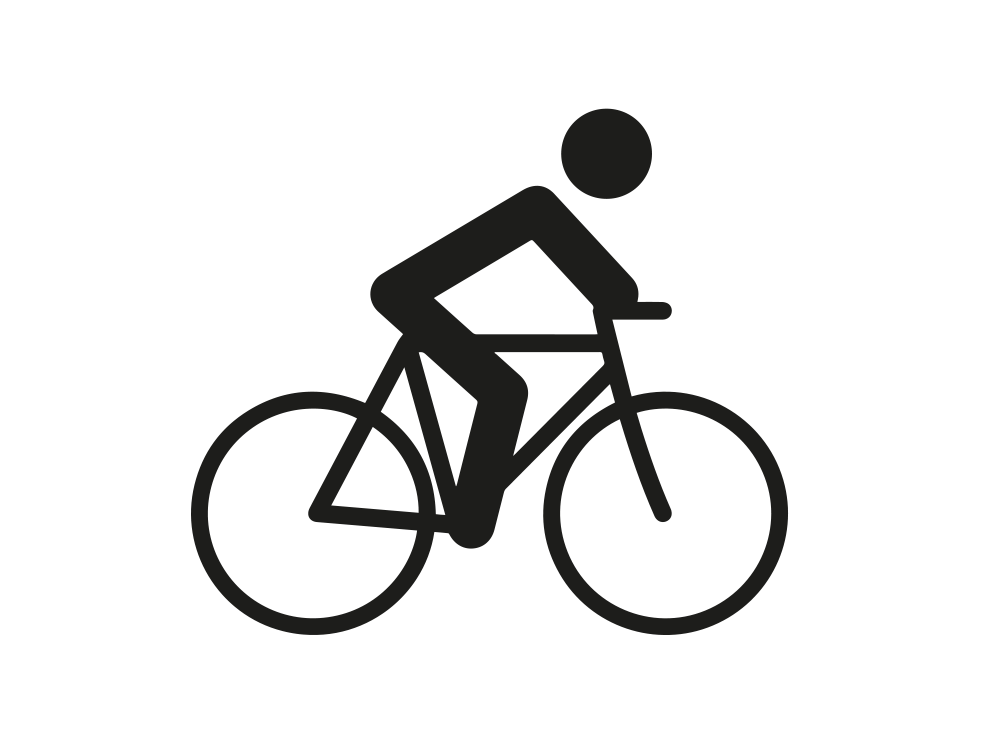
\includegraphics[scale = 0.2]{media/images/velo}
		\end{center}
		\vspace{2 cm}
		\begin{minipage}{0.75\textwidth}
			\begin{flushleft}
				SPELGATTI Andrea \\
				Alexandre Gallez \\
				Master Ingénieur Industriel | M18\\
				Année 2022-2023
			\end{flushleft}
		\end{minipage}
		\vspace{3cm}
		\begin{center}
			{\bfseries \today}
		\end{center}
\end{titlepage}
%
\null
%\newpage %used if having a page de garde

%\pagenumbering{roman} % numérotation en chiffres romains
%\setcounter{page}{1}

%\addcontentsline{toc}{chapter}{Résumé}
\chapter*{Résumé} 


Résumé ici

\begin{singlespace}
\textbf{Mots clés~:} Mots-clés ici
\end{singlespace}
%\addcontentsline{toc}{chapter}{Abstract}
\chapter*{Abstract}
\selectlanguage{english}
Abstract

\begin{singlespace}
\textbf {Keywords ~:} keywords
\end{singlespace}
\selectlanguage{french}
%\addcontentsline{toc}{chapter}{Remerciements}
\chapter*{Remerciements} 


Je remercie...

Rappelez-vous de remercier \LaTeX

\begin{singlespace}
    \selectlanguage{french}
    \tableofcontents % table des matières
    %\listoffigures % si vous avez des images... si vous n'en avez pas, effacez cette ligne
\end{singlespace}

% fin numérotation en chiffres romains
% début numérotation en chiffres arabs3
\pagenumbering{arabic}
\setcounter{page}{0}


%dans les fichier vous trouverez des exemples d'usage des différentes commandes de LaTeX
\begin{onehalfspace}
\thispagestyle{empty}
   	\chapter{Layer 1 - Hardware}
\section{Raspberry Pi}
\section{ESP32}
\section{ESP8266}
   	\chapter{Layer 2 - Interface Utilitaire}
   	\chapter{sécurité}
\section{mot de passe}

 nous avons pris des mesures rigoureuses. Les mots de passe ont été stratégiquement appliqués à divers niveaux de notre système, notamment sur les connexions SSH, Node-RED et MongoDB. Cette approche multicouche renforce la confidentialité des données, prévenant tout accès non autorisé et assurant une expérience utilisateur sûre et protégée à chaque étape.
 
\section{Sécuriser les communications}

nous avons adopté une approche intégrée. Les communications au sein de notre système sont désormais protégées par des certificats de sécurité pour MQTT, MongoDB et Node-RED. Ces certificats agissent comme des boucliers numériques, garantissant la confidentialité des échanges et prévenant toute intrusion non autorisée


\section{API et applications externes utilisées}

chaque requête API est étroitement surveillée et protégée par des tokens de connexion. Ces tokens agissent comme des gardiens numériques, permettant uniquement l'accès autorisé aux informations sensibles. Cette stratégie de sécurité robuste garantit que seules les interactions légitimes ont accès.

\section{Docker}

 nous avons opté pour Docker en tant qu'outil de protection supplémentaire. Les conteneurs Docker offrent une isolation rigoureuse pour chaque application et service, empêchant la propagation de vulnérabilités potentielles.
   	\chapter{conclusion}


\section{Alexandre}
\subsection{ niveau de connaissance avant }
\begin{itemize}
    \item en développement: java script et python  mon niveau se reposait sur mes connaissances d'algorithmie.

    \item je ne connaissais pas node red avant de commencer le projet.

    \item en électronique: je connaissais bien le fonctionnement de composant électronique.

    \item en système : j'avais de bonnes connaissances en linux 
 \end{itemize}    
\subsection{niveau de connaissance après le projet }
\begin{itemize}
    \item en développement java script , j'ai appris à utiliser node js , le gestionnaire de package npm , ainsi que pas mal de notions spécifiques a la programmation java script.

    \item en python, j'ai appris à utiliser de nombreuses librairies, ainsi, j'ai appris une partie du style de programmation.
    
   \item je maîtrise globalement node red. 

    \item en électronique, j'ai consolidé mes connaissances sur comment fonctionnent certains capteurs. 

    \item en système : j'ai renforcé mes connaissances en configurations de fichiers , comment fonctionne le système d'exploitation et les services.

   \item suite à de nombreux bugs , j'ai également amélioré ma connaissance de git. 
    
    \item j'ai appris aussi à mieux comprendre comment résoudre tout type d'erreurs.

 \end{itemize}    
\subsection{les difficultés rencontrés}
\begin{itemize}
    \item problèmes d'horloge avec le Raspberry pi, ce qui a engendré des problèmes de git et d'installation de package.
    \item énorme problème d'utilisation du Bluetooth qui nous a contraint à rechanger toute notre architecture initiale. 
    \item problème de pi Cam , après de nombreuses tentatives , il s'avère que le problème était hardware.
    \item problème de librairie python l'import de grouvepi ne s'effectuait pas correctement
    \item problème pour comprendre comment injecter un point sur worldmap , il fallait mettre le payload en format json et non en string comme tous les autres nodes.
    \item difficulté à comprendre le fonctionnement de certains capteurs
    \itemproblème d'interaction avec esp8266.
    

 \end{itemize}
\section{Andrea}
\subsection{ Connaissance avant projet }
    \begin{itemize}
        \item Base intermédiaire en linux -> systemd/gestion des droits
        \item Cours de microcontrolleur pour ce qui est des esp
        \item Docker Intermédiaire
        \item Débutant Python
        \item Débutant Javascript/NodeJS
        \item Base de git
        \item Aucune connaissance préalable sur mqtt/nodejs/no-sql
    \end{itemize}
\subsection{ Connaissance Post-projet }
     \begin{itemize}
        \item Base intermédiaire en linux -> Amélioration de la compréhension systemd/gestion des droits 
        \item Cours de microcontrolleur pour ce qui est des esp utilisation réel de certaines notions
        \item Docker Intermédiaire -> utilisation plus poussée des volumes et de compose
        \item Débutant Python -> Amélioration notable
        \item Débutant Javascript/NodeJS -> Connaissance de base + NPM qui permet de faire des choses intéressantes très rapidement
        \item Base de git -> problem solving dû à des probléme d'horloges
        \item Aucune connaissance préalable sur mqtt/nodejs/no-sql, Introduction comprise et mon intérêt est présent.
    \end{itemize}
\subsection{les difficultés rencontrées}
J'ai eu moins de temps sur le projet que Alexandre, je suis donc souvent intervenu lors de problème qui bloquait depuis longtemps.
\begin{itemize}
    \item Bulleyes -> nous avons installé la version le plus récent de raspian ça a causé de nombreux problèmes aux niveaux de l'installation de grove pi. On a dû donc trouvé des fix en cherchant beaucoup.
    \item Le time gate, l'horloge de la raspberryPi n'était pas à jour suite à des problèmes avec NTP.
    On a dû fix de nombreux problèmes suite à ça :
    \begin{itemize}
        \item git qui buguait complétement,
        \item nodered ne savait plus installer d'addons
        \item le script d'installation officiel de nodered ne fonctionnait pas → installation de nodered via NPM
    \end{itemize}
    \item Connexion LORA plein d'artefact, ajout d'un CRC à la main
    \item Communication compliquée entre le serveur et la rpi → utilisation d'un VPN local pour éviter des problèmes de changement d'ip et permettre le travail à distance
    \item Problème de droit lors du lancement de nodejs via systemd, en effet nous n'avions pas ajouté les droits d'accès aux gpio à l'utilisateur nodered.
    \item Problème de firewall, configuration de firewalld
    \item Problème étrange de lecture des certificats générés, où les serveurs ne savait pas les lires -> fix avec un script d'installation.
    \item Probablement plein de petit problèmes intermédiaires, dont je ne me rappelle pas..
\end{itemize}
\subsection{Conclusion personnelle sur le projet}
Le projet m'a vraiment intéressé et j'ai aimé pouvoir jouer avec toutes ses technologies, mais le fait de devoir incorporer des technologies et fonctionnalité pas réellement nécessaire au projet. Dans un objectif de dire qu'on l'a fait, a réduit mon enthousiasme. 

J'aurais apprécié un peu plus de liberté dans le projet.

La parenthèse conclue, je compte réutiliser mqtt si j'en ai l'occasion, et continuer à utiliser des rpi pour héberger de petits projets rapidement, et ça m'a donné envie de m'intéresser à la domotique.
\end{onehalfspace}


% Here you should put bibliography related content
\printbibliography



\end{document} 